
\section{Testovací prostředí}
Veškeré provedené testy proběhly na lokálním počítači s operačním systémem Ubuntu 16.04,
na kterém zároveň proběhl vývoj nástroje. Systémové
prostřekdy dostupné pro testovaní byly: 4 jádra CPU, 8 GB RAM, 17 GB SSD disk.

Na počítači byl nasazen systém NEMEA a IoT brána BeeeOn, která byla rozšířena o vytvořený detekční 
nástroj. Pro generování senzorových dat byly použity následující zařízení: BLE teplotní senzor (BeeWi), 
Z-Wave zásuvka (POPP) a virtuální senzory, které jsou dostupné pro testování na BeeeOn bráně.

\section{Způsoby nasazení}
Jako první byly testovány možnosti nasazení vytvořeného nástroje, který je možné používat v 
následujících režimech:

 \begin{itemize}
  \item \textbf{Lokální režim}
  
  V lokální variantě byl použit pouze modul detektoru a kolektoru. Aby se nemusela pro každou 
  událost spouštět nová instance detektoru, byl využit již existující NEMEA modul \textit{Merger},
  který 
  dokáže jendotlivé UniRec zprávy spojit do jedné konsolidované. Způsob nasazení je na obrázku 
  \ref{obr.option1}.
  \begin{figure}[ht]
   \begin{center}
   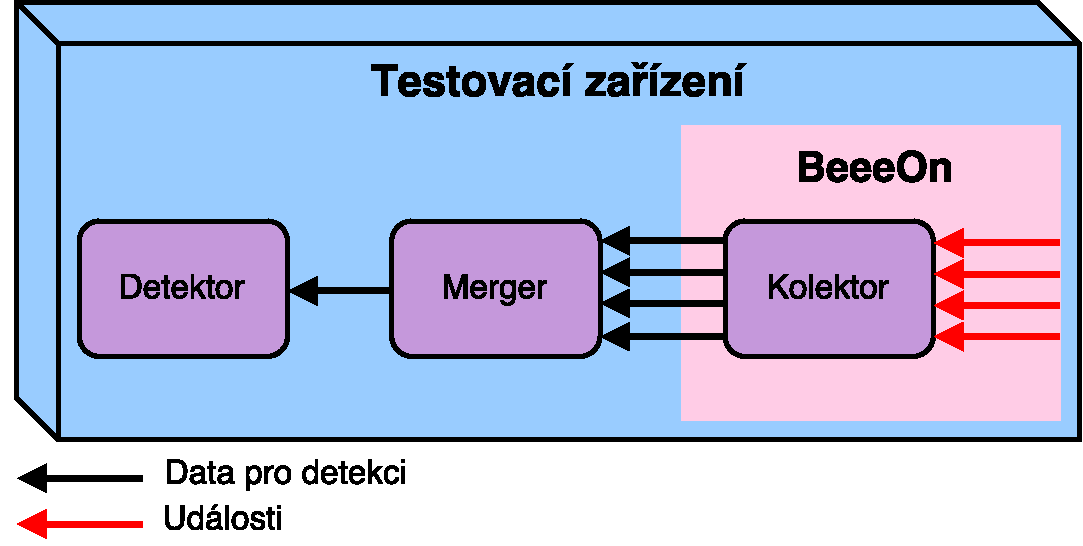
\includegraphics[scale=0.5]{pictures/deploy-option1}
   \caption{Lokální nasazení}
   \label{obr.option1}
   \end{center}
   \end{figure}
   
   Kolektor odesílá vždy dostupné události specifikovanými výstupními rozhraními dle konfigurace brány.
   Exporovaná data přijímá NEMEA modul \textit{Merger}, který je spojuje a předává detektoru.
   
  \item \textbf{Oddělený režim}
  
  Druhý způsob nasazení byl také otestován na lokálním zařízení, protože lze možné využít lokálních
  soketů, které nabízí NEMEA framework. Způsob zavedení je na obrázku \ref{obr.option2}.
 
  \begin{figure}[ht]
   \begin{center}
   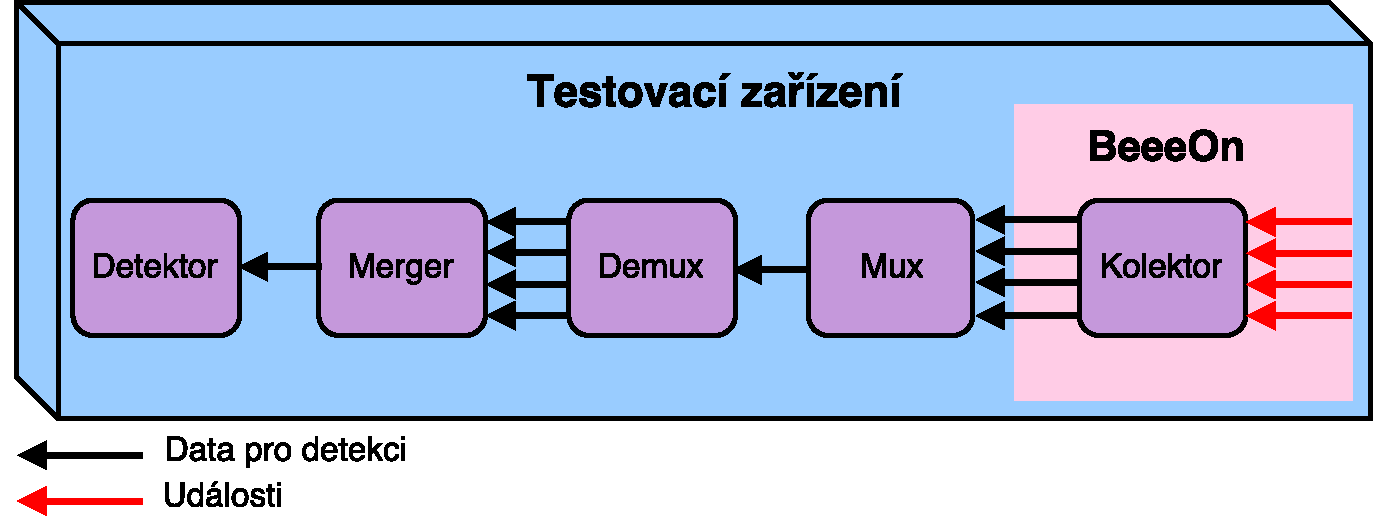
\includegraphics[scale=0.5]{pictures/deploy-option2}
   \caption{Oddělené nasazení}
   \label{obr.option2}
   \end{center}
   \end{figure}
   
   Složení komponent vychází z prvního případu, který byl rozšířen o moduly Mux a Demux, které 
   umí spojit a rozdělit přicházející komunikaci.
 \end{itemize}
 
Cílem testů je, aby detektor obdržel všechny odeslané zprávy z kolektoru. Ověření bylo provedeno
spuštěním detektoru s přepínačem \textit{-vv}, který zapne ladící výpisy druhé úrovně pro zobrazení 
přijatých UniRec polí. Výsledky obou případů byly úspěšné a všechna data byla přijata.

\section{Detekce scénářů útoků}
Velmi důležitou částí bylo otestování definovaných anomálií, které mohou reprezentovat skutečný
útok na sít. Tato sekce popisuje testy pro jednotlivé scénáře.

  \begin{enumerate}
    \item \textbf{Periodicita dat}
    \item \textbf{Množství přenášených zpráv}
    \item \textbf{Limity senzorových hodnot}
    \item \textbf{Kvalita přenosového kanálu}
    \item \textbf{Konektivita}
  \end{enumerate}

%popis otestování scénářů
\section{Test ostatních funkcionalit}
Vytvořený detekční systém obsahuje i další funcionality, které nebyly použity v definovaných scénářích,
ale mohou být užitečné pro budoucí používání. Tato sekce obsahuje testy pro zbylé možnosti
detekce.

%test ostatních funcionalit, které jsem doplnil, export, ....